\section{Алгоритм Обучи}
\label{sec:base}

Лучшим в смысле устойчивости к атакам из известных автору алгоритмов является алгоритм предложенный 
Ohbuchi et al. в работе \cite{Ohbuchi}. Это хорошо информированный, работающий в частотной области алгоритм,
главная идея которого заключается в применении техники, разработанной для трехмерной полигональной сетки к
двумерным картам.
Для вычисления частотного представления планарного графа строится его триагуляция Делоне с ограничениями 
(\cite{Chew}), и для получившейся сетки вычисляется частотное представление, используя спектральный анализ 
предложенный в работах \cite{Karni1, Karni2}. Затем частотные коэффициенты изменяются согласно битам 
внедряемого сообщения. Обратным преобразованием модифицированных коэффициентов в координаты вершин получается
карта с внедренными водяными знаками. Изменение коэффициенто в частотной области влечет смещение вершин в 
пространственной области.

Для увеличения эффективности вычислений и устойчивости против обрезки карта вначале делится на прямоугольные 
области содержащие примерно одинаковое количество вершин (рис. \ref{pic_ohbuchi}). 
\begin{figure}
  \centering
  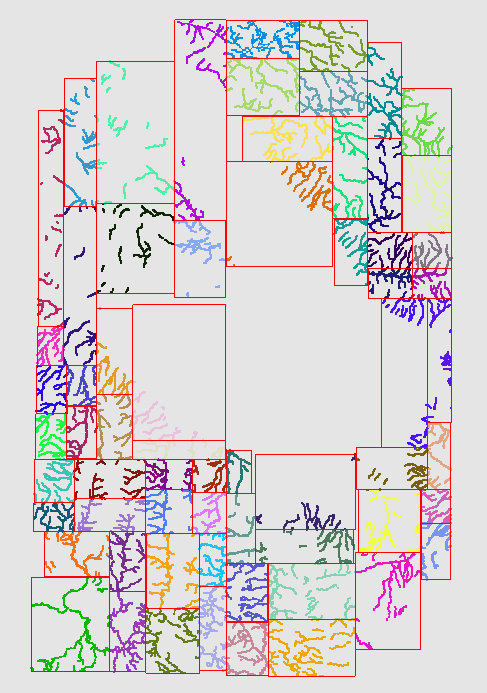
\includegraphics[scale=1.0]{ohbuchi.png}
  \caption{Разбиение карты на области}
  \label{pic_ohbuchi}
\end{figure}
Упомянутые выше спектральный анализ и внедрения водяных знаков производится для каждой области независимо.

Водяные знаки извлекаются сранением орининальной и атакованной карты. В первую очередь карты геометрически
''регистрируются'' с помощью итеративного процесса минимизации расстояния между множествами предварительно
выбранных пометок. Эта регистрация может устранить аффинное преобразование примененное к подписанной карте.

Для вставки вершин удаленных злоумышленником и удаления вершин вставленных злоумышленников используется 
следующий алгоритм. Для каждой вершины оригинальной
карты осуществляется поиск вершин в круге некоторого радиуса на атакованной карте. Если не было найдено ни одной,
вершины то соответсвующая вершина добавляется, если было найдено несколько, то удаляются все кроме ближайшей
к соответствующей вершине оригинальной карты.

Рассмотрим процесс внедрения ЦВЗ подробнее.  
Пусть $V = \{v_1, v_2, \dots, v_n\}$ есть множество вершин оригинальной карты, $n = |V|$. 
Пусть $\mathfrak{T}$ озбозначает некоторую триангуляцию множества $V$, $G(\mathfrak{T})$ обозначает 
граф триангуляции $\mathfrak{T}$. Собственные вектора $\{\mathbf{e}_i\}_{i=1}^n$ графа $G(\mathfrak{T})$ суть 
собственные вектора его лапласиана. 
Существует несколько определений лапласиана графа, к примему \cite{Biggs, Chung, Zhang}. В базовом алгоритме 
используется определение данное в \cite{Biggs}
$$R = I - D^{-1} A,$$ где $I$ --- единичная матрицв, $D$ --- диагональная матрица составленная из 
степеней вершин графа $G(\mathfrak{T})$, $A$ --- матрица смежности $G(\mathfrak{T})$
\begin{eqnarray*}
  D_{ij} = \begin{cases} deg(v_i) &\text{if $i = j$,} \\ 0 &\text{otherwise;} \end{cases} \\
  A_{ij} = \begin{cases} 1 &\text{if vertices $i$ and $j$ is adjacent,} \\ 0 &\text{otherwise.} \end{cases} 
\end{eqnarray*}
Собственные вектора $\{\mathbf{e}_i\}_{i=1}^n$ составляют базис $\mathbb{R}^n$. Будем предполагать, что 
собственные вектора нормализованны, $||e_i|| = 1$. 
Пусть $v_i = (x_i, y_i)$ тогда $\mathbf{r} = (r_1, r_2, \dots, r_n)$, $\mathbf{s} = (s_1, s_2, \dots, s_n)$ 
суть разложения векторов $\mathbf{x} = (x_1, x_2, \dots, x_n)^T$, $\mathbf{y} = (y_1, y_2, \dots, y_n)^T$ 
соответственно в базисе $\{\mathbf{e}_i\}_{i=1}^n$. Другими словами 
\begin{eqnarray*}
  \mathbf{x} = r_1 \mathbf{e}_1 + r_2 \mathbf{e}_2 + \dots + r_n \mathbf{e_n}; \\ 
  \mathbf{y} = s_1 \mathbf{e}_1 + s_2 \mathbf{e}_2 + \dots + s_n \mathbf{e_n}.  
\end{eqnarray*}
Если $\{\mathbf{e}_i\}_{i=1}^n$ ортогональны, то $r_i = (\mathbf{x}, \mathbf{e}_i)$, 
$s_i~=~(\mathbf{y}, \mathbf{e}_i)$, но в общем случае это не верно. 

Предположим, что внедряемое сообщение $\mathbf{m} = (m_1, m_2, \dots, m_k)$ состоит из $k$ бит, где $k \le n$, 
$m_i \in \{0, 1\}$. Введем обозначение $q_i = 2 * m_i - 1$, $q_i \in \{-1, 1\}$.
Изменим коэффициенты $r_i, s_i$, $1 \le k \le n$ следующим образом
\begin{eqnarray*}
  r_i' = r_i + \alpha p_i q_i; \\
  s_i' = s_i + \alpha p_i q_i, 
\end{eqnarray*}
где $\{p_i\}$ есть псевдослучайная последовательность, $\alpha$ --- некоторая положительная константа. 
Увеличение ~$\alpha$ увеличивает устойчивость к атакам на внедренные ЦВЗ, но вызывает большее искажение
карты. 

Пусть $\mathbf{x'}, \mathbf{y'}$ координаты вершин подписанной карты. 
\begin{eqnarray*}
  \mathbf{x'} - \mathbf{x} = (r_1' - r_1) \mathbf{e}_1 + (r_2' - r_2) \mathbf{e}_2 + \dots + (r_n' - r_n) \mathbf{e_n} = \\
  = \alpha \left[ p_1 q_1 \mathbf{e}_1 + p_2 q_2 \mathbf{e}_2 + \dots + p_k q_k \mathbf{e}_k \right], \\
  \mathbf{y'} - \mathbf{y} = \alpha \left[ p_1 q_1 \mathbf{e}_1 + p_2 q_2 \mathbf{e}_2 + \dots + p_k q_k \mathbf{e}_k \right]. 
\end{eqnarray*}
Другими словами внедрение ЦВЗ может быть выражено как построение вектора  
\begin{equation}
\label{formula:g}
 \mathbf{g} = \alpha \left[ p_1 \mathbf{h}_1 + p_2 \mathbf{h}_2 + \dots + p_k \mathbf{h}_k \right]; 
\end{equation}
$$ \mathbf{h_i} = \left( \begin{pmatrix} e_{i, 1} \\ e_{i, 1} \end{pmatrix} 
\begin{pmatrix} e_{i, 2} \\ e_{i, 2} \end{pmatrix}, \dots, \begin{pmatrix} e_{i, n} \\e_{i, n}  \end{pmatrix} 
\right), 1 \le i \le n. $$
Если вектора $\{\mathbf{e}_i\}_{i=1}^n$ ортонормированны, можно оценить среднее по всем вершинам расстояние 
смещения $\Delta v_{mean}$.
\begin{equation}
\label{formula:mean_displacement}
|\mathbf{g}| = \alpha * \sqrt {k} * \sqrt{2}; \mbox{      } \Delta v_{mean} = \alpha * \frac{\sqrt{2k}}{n}. 
\end{equation}

Для извлечение водяных знаков необходимо разложить вектора $\mathbf{x'} - \mathbf{x}$, 
$\mathbf{y'} - \mathbf{y}$ в базисе $\{\mathbf{e}_i\}_{i=1}^k$, то есть вычислить коэффициенты 
$\mathbf{u} = (u_1, u_2, \dots, u_k)$, $\mathbf{w} = (w_1, w_2, \dots, w_k)$, 
\begin{eqnarray*}
  \mathbf{x'} - \mathbf{x} = u_1 \mathbf{e}_1 + u_2 \mathbf{e}_2 + \dots + u_k \mathbf{e_k}; \\ 
  \mathbf{y'} - \mathbf{y} = w_1 \mathbf{e}_1 + w_2 \mathbf{e}_2 + \dots + w_k \mathbf{e_k}.  
\end{eqnarray*}
Биты внедренного сообщения получаются так:
$$q_i = \sgn(p_i * (u_i + w_i)), m_i = (q_i + 1) / 2.$$
